% Options for packages loaded elsewhere
\PassOptionsToPackage{unicode}{hyperref}
\PassOptionsToPackage{hyphens}{url}
%
\documentclass[
]{article}
\usepackage{lmodern}
\usepackage{amssymb,amsmath}
\usepackage{ifxetex,ifluatex}
\ifnum 0\ifxetex 1\fi\ifluatex 1\fi=0 % if pdftex
  \usepackage[T1]{fontenc}
  \usepackage[utf8]{inputenc}
  \usepackage{textcomp} % provide euro and other symbols
\else % if luatex or xetex
  \usepackage{unicode-math}
  \defaultfontfeatures{Scale=MatchLowercase}
  \defaultfontfeatures[\rmfamily]{Ligatures=TeX,Scale=1}
\fi
% Use upquote if available, for straight quotes in verbatim environments
\IfFileExists{upquote.sty}{\usepackage{upquote}}{}
\IfFileExists{microtype.sty}{% use microtype if available
  \usepackage[]{microtype}
  \UseMicrotypeSet[protrusion]{basicmath} % disable protrusion for tt fonts
}{}
\makeatletter
\@ifundefined{KOMAClassName}{% if non-KOMA class
  \IfFileExists{parskip.sty}{%
    \usepackage{parskip}
  }{% else
    \setlength{\parindent}{0pt}
    \setlength{\parskip}{6pt plus 2pt minus 1pt}}
}{% if KOMA class
  \KOMAoptions{parskip=half}}
\makeatother
\usepackage{xcolor}
\IfFileExists{xurl.sty}{\usepackage{xurl}}{} % add URL line breaks if available
\IfFileExists{bookmark.sty}{\usepackage{bookmark}}{\usepackage{hyperref}}
\hypersetup{
  pdftitle={WasteWater Analysis},
  pdfauthor={Steve Goldstein and Marlin Lee},
  hidelinks,
  pdfcreator={LaTeX via pandoc}}
\urlstyle{same} % disable monospaced font for URLs
\usepackage[margin=1in]{geometry}
\usepackage{graphicx,grffile}
\makeatletter
\def\maxwidth{\ifdim\Gin@nat@width>\linewidth\linewidth\else\Gin@nat@width\fi}
\def\maxheight{\ifdim\Gin@nat@height>\textheight\textheight\else\Gin@nat@height\fi}
\makeatother
% Scale images if necessary, so that they will not overflow the page
% margins by default, and it is still possible to overwrite the defaults
% using explicit options in \includegraphics[width, height, ...]{}
\setkeys{Gin}{width=\maxwidth,height=\maxheight,keepaspectratio}
% Set default figure placement to htbp
\makeatletter
\def\fps@figure{htbp}
\makeatother
\setlength{\emergencystretch}{3em} % prevent overfull lines
\providecommand{\tightlist}{%
  \setlength{\itemsep}{0pt}\setlength{\parskip}{0pt}}
\setcounter{secnumdepth}{-\maxdimen} % remove section numbering

\title{WasteWater Analysis}
\author{Steve Goldstein and Marlin Lee}
\date{6/1/2021}

\begin{document}
\maketitle

Focus on HF Data.

replicates and our best shot.

Cases: larger pop avoids problematic small pop areas (low numbers have a
lot of variance; 1-4 =\textgreater{} -999. also: relatively small sample
size (relative to variance in case counts): short duration; some flowage
districts have fewer observations. Describe plots of cases (or
\%positive): Unimodal: is there a trend? segmentation? can't say; Cases
plot:

\includegraphics{WasteWaterAnalysis_files/figure-latex/No claer relation Cases-1.pdf}

\includegraphics{WasteWaterAnalysis_files/figure-latex/Case comp-1.pdf}
\includegraphics{WasteWaterAnalysis_files/figure-latex/Case comp-2.pdf}

\begin{verbatim}
##      Site       Date CollectedCases Cases
## 1 Madison 2021-01-19            138    36
## 2 Madison 2021-01-28             88   204
## 3 Madison 2021-02-02            138    46
## 4 Madison 2021-02-04             72   169
## 5 Madison 2021-02-16            130    33
## 6 Madison 2021-02-27             38   142
\end{verbatim}

\begin{verbatim}
##      Site       Date ConfirmedCases Cases
## 1 Madison 2021-01-15             12   117
## 2 Madison 2021-01-27            163    71
## 3 Madison 2021-01-28             97   204
## 4 Madison 2021-02-03            160    65
## 5 Madison 2021-02-04             93   169
## 6 Madison 2021-02-27             35   142
\end{verbatim}

N1: left (and right?): outliers called out by Dagmara; action: ignore
them. remaining dips: what are they: 3 interpretations:

\begin{enumerate}
\def\labelenumi{(\alph{enumi})}
\item
  real dip;
\item
  just chaotic quirky;
\item
  longer explanation: 9 replicates have low var; OK good experiment;
  good benchwork. now think about the stochasticity of the sampling
  process; you capture a liter of ww whose N1 concentration is a random
  variable.
\end{enumerate}

\includegraphics{WasteWaterAnalysis_files/figure-latex/No clear relation N1-1.pdf}

\%BoCov and PMMOV can we use these? answer: don't see how.

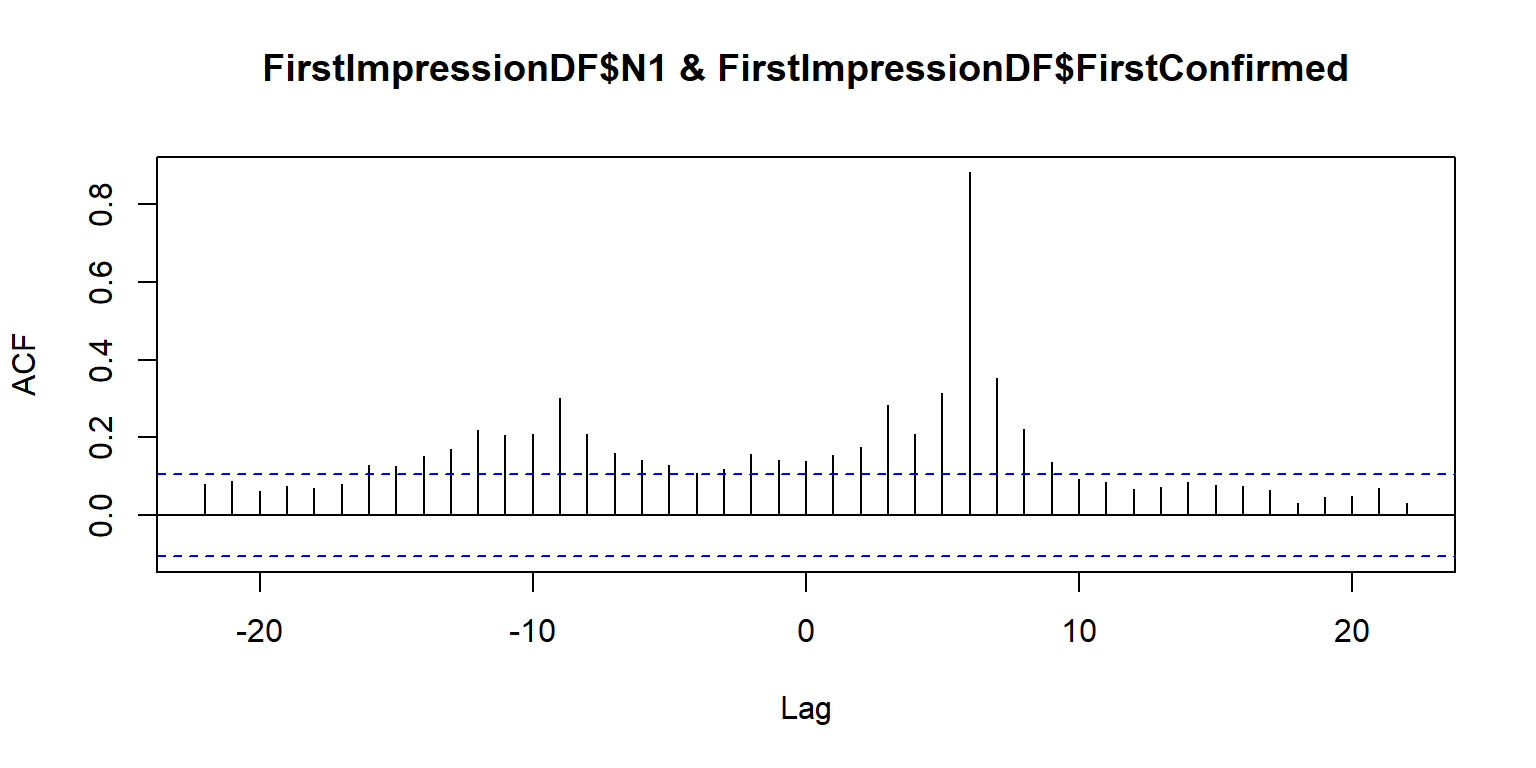
\includegraphics{WasteWaterAnalysis_files/figure-latex/unnamed-chunk-1-1.pdf}
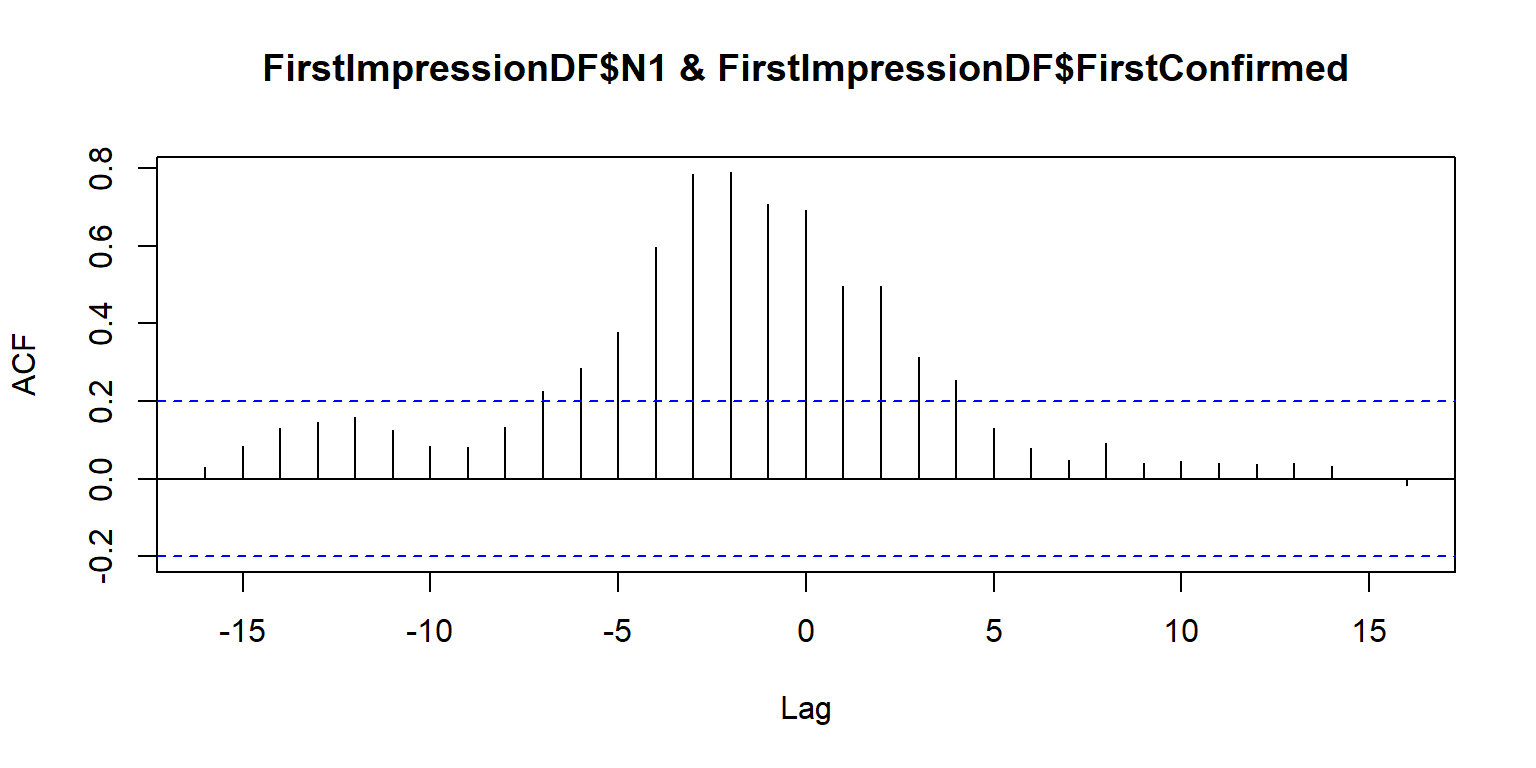
\includegraphics{WasteWaterAnalysis_files/figure-latex/unnamed-chunk-1-2.pdf}

\includegraphics{WasteWaterAnalysis_files/figure-latex/outliers Per_Bcov-1.pdf}
\includegraphics{WasteWaterAnalysis_files/figure-latex/outliers Per_Bcov-2.pdf}

question to resolve: date off by one between MMSD and HFG; is it in the
emails or READMEs?

\includegraphics{WasteWaterAnalysis_files/figure-latex/madison messure same data-1.pdf}

UW thresholding / box plots

\includegraphics{WasteWaterAnalysis_files/figure-latex/boxplots-1.pdf}

\end{document}
